\begin{activity}\label{A:0.2.1}
    Consider the exponential functions plotted in Figure \ref{F:0.2.Act1}
    \ba
        \item Which of the functions have common ratio $r > 1$?
        \item Which of the functions have common ratio $0<r< 1$?
        \item Rank each of the functions in order from largest to smallest $r$ value.
    \ea
    \begin{figure}[h!]
        \begin{center}
%             \begin{tikzpicture}
%                 \begin{axis}[axis lines=center, xlabel={$x$}, ylabel={$y$}, xmin=-3, xmax=3,
%                     ymin=-1, ymax=5, domain=-3:3,legend pos=outer north east]
%                     \addplot[smooth, blue, very thick] {2^x};
%                     \addlegendentry{$f(x)$};
%                     \addplot[smooth, red, very thick, dashed] {3^x};
%                     \addlegendentry{$g(x)$};
%                     \addplot[smooth, green!50!black, very thick, dotted] {1.5^x};
%                     \addlegendentry{$h(x)$};
%                     \addplot[smooth, black, very thick, dashdotted] {(0.5)^x};
%                     \addlegendentry{$k(x)$};
%                     \addplot[smooth, cyan, very thick, densely dotted] {(0.9)^x};
%                     \addlegendentry{$m(x)$};
%                 \end{axis}
%             \end{tikzpicture}
            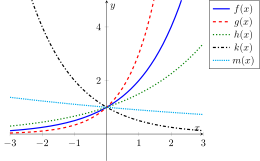
\includegraphics[width=0.6\columnwidth]{figures/0-2-figAct1.pdf}
        \end{center}
        \caption{Exponential growth and decay functions} \label{F:0.2.Act1}
    \end{figure}
\end{activity}
\begin{smallhint}
   \ba
        \item If the common ratio is larger than 1 what will happen to the $y$ values?
            For example, if the common ratio were 2 and we start with 5 then what would
            the next value be?
        \item If the comon ratio is less than 1 what will happen to the $y$ values?
        \item Do some experimentation to determine which ones will be steeper or less
            steep.
   \ea
\end{smallhint}
\begin{bighint}
   \ba
        \item If we start with 5 and the common ratio is 2 then the next value would be
            10, then 20, then 40, etc.
        \item If we start with 5 and the common ratio is $1/2$ then the next value would
            be $5/2$, then $5/4$, then $5/8$, etc.
        \item The exponential growth functions that grow fastest have the larger common
            ratio.
   \ea
\end{bighint}
\begin{activitySolution}
   \ba
        \item blue, red, dark green
        \item cyan and black
        \item blue is $y = 2^x$, red is $y = 3^x$, dark green is $y=1.5^x$, cyan is
            $y=0.9^x$, and black is $y=0.5^x$.
   \ea
\end{activitySolution}

\aftera
